\scanpage{68}
À \deleted{prouver que}\inserted{définir un} isom de foncteurs
\[
(\unsure{A|\alpha})\qquad \mathbb{R}i^!\simeq
\deleted{\unsure{(\mathbb{R}^!g)}}\,\mathbb{R}^{\deleted{\unsure{!}}}(j\sigma)^!\mathbb{R}^!g
\]
et une commutativité de diagrammes reliant les $\operatorname{Tr}_i$\deleted{\unsure{et}}, $\operatorname{Tr}_g$, $\operatorname{Tr}_{j\sigma}$.
Comme on a un isom
\[
\mathbb{R}(j\sigma)^!\simeq \mathbb{R}\sigma^!\,\mathbb{R}j^!
\]
provenant de
\[
(j\sigma)^!\simeq\sigma^!j^!
\]
on définira $(\unsure{A|\alpha})$ comme \deleted{déduit de}
\[
\mathbb{R}^{\deleted{\unsure{!}}}\deleted{\unsure{\sigma}}i^!
\simeq \mathbb{R}^{\deleted{\unsure{!}}}\sigma^!(\mathbb{R}j^!\,\mathbb{R}^!g)
\]
déduit des isom suivants
\[
\left\{\begin{aligned}
(\mathbb{R}^!\unsure{g'})(\mathbb{R}i^!)&\simeq(\mathbb{R}^{\deleted{\unsure{!}}}j^!)(\mathbb{R}^!g) &&(a)\\
\deleted{\unsure{\mathbb{R}^!\operatorname{id}_{\mathrm D^+(Y')}}}\quad
\mathbb{R}^!\operatorname{id}_{Y'}&\simeq(\mathbb{R}\sigma^!)(\mathbb{R}^!g') &&(b)
\end{aligned}\right.
\]
d'où
\[
\begin{aligned}
\mathbb{R}i^!&=\deleted{\unsure{(\mathbb{R}i^!)}}
(\mathbb{R}^!\operatorname{id}_{Y'})(\mathbb{R}i^!)
\underset{\inserted{\text{après : $(a)$}}}{\simeq}
\deleted{\unsure{\mathbb{R}i^!}}\mathbb{R}\sigma^!\,
\underbrace{\mathbb{R}^!g'\,\mathbb{R}i^!}_{\deleted{\unsure{(a)}}}\\
&\simeq
\inserted{\text{\figure{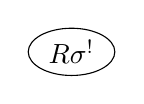
\begin{tikzpicture}[baseline=-.5ex]
\draw (0,0) ellipse (.55 and .3);
\node at (0,0) {$\mathbb{R}\sigma^!$};
\end{tikzpicture}}}}
(\mathbb{R}j^!\,\mathbb{R}^!g\,\deleted{\unsure{\mathbb{R}i^!}})
\end{aligned}
\]
ce qu'on voulait définir. Il faut donc définir $(a)$ et $(b)$. Or $(b)$ est un cas particulier du ``th. de compatibilité des classes fond locales et globales'' (lorsque l'un des \unsure{$Y$-schémas} \unsure{lisses envisagés} est isom. à la base \unsure{\ldots}).
\mspage{67}
